\documentclass[9pt,hyperref={pdfpagelabels=false},xcolor=table]{beamer}
\usepackage{multicol}

% Contact information: 
%   Jorge M. Cruz-Duarte (jorge.cruz@tec.mx)
%   Nov. 29, 2019

\usepackage{lmodern, ragged2e, CJKutf8, booktabs, subfig,adjustbox, graphicx, amsmath, amssymb, amsthm, amsfonts, mathtools, multirow,wrapfig,lipsum,tikz, tikz-cd,tikz-3dplot,pgfplots}
\usetikzlibrary{shapes.geometric}
% \usepackage{amsmath, amsthm, amssymb, amsfonts, amsthm, bbold, bm}
\usepackage[alpine,misc,geometry,electronic]{ifsym}
\usepackage[style=phys]{biblatex}
\usepackage[lined,boxed,vlined,ruled,linesnumbered]{algorithm2e}
\SetKw{Continue}{continue}
\SetKw{Or}{or}
\SetKw{Until}{until}
\addbibresource{bibliography.bib}
\renewcommand{\footnotesize}{\tiny}
\newcommand{\norm}[1]{\left\lVert#1\right\rVert}
\makeatletter
\@newctr{footnote}[page]
\makeatother

\usetheme{CambridgeUS}
\renewcommand{\raggedright}{\leftskip=0pt \rightskip=0pt plus 0cm}

\definecolor{UQPurple}{RGB}{0, 32, 159}
% This is the trademark pruple that UQ uses
\definecolor{UQPurple}{RGB}{81,36,122}
\newcommand{\hl}[1]{{\textcolor{UQPurple}{#1}}}

% Theme setup
\titlegraphic{\includegraphics[scale=0.05]{img/UQ_color_logo.png}}

% \makeatletter
\setbeamertemplate{headline}{%
  \leavevmode%
  \hbox{%
    \begin{beamercolorbox}[wd=\paperwidth,ht=2.5ex,dp=1.125ex]{palette quaternary}%
      \insertsectionnavigationhorizontal{\paperwidth}{}{\hskip0pt plus1filll}
    \end{beamercolorbox}%
  }
}
\setbeamertemplate{footline}{\hspace*{2ex} \insertshortauthor \hfill \textcolor{UQPurple}{\insertshorttitle} \hfill \textbf{\insertframenumber{}} / \inserttotalframenumber \hspace*{2ex}}

\setbeamercolor{item projected}{bg=UQPurple}
\setbeamertemplate{enumerate items}[default]
\setbeamercolor*{enumerate item}{fg=UQPurple}

\setbeamertemplate{navigation symbols}{}
% \setbeamertemplate{footline}[\insertshorttitle frame number]
\setbeamertemplate{bibliography item}[text]
\setbeamertemplate{theorems}[numbered]

\setbeamerfont{title}{series = \bfseries, parent = structure}
\setbeamerfont{frametitle}{series = \bfseries, parent = structure}
\setbeamerfont{headline}{series = \bfseries, size = \tiny, parent = structure}

\setbeamercolor{title}{fg = white, bg = UQPurple}
\setbeamercolor{frametitle}{fg = white, bg = UQPurple}
\setbeamercolor{structure}{fg = UQPurple}
\setbeamercolor{section in head/foot}{fg = black, bg = UQPurple!40}
\setbeamercolor{subsection in head/foot}{fg = black, bg = UQPurple!20}

\setbeamercolor{block title}{use=structure,fg=white,bg=structure.fg!75!black}
\setbeamercolor{block body}{parent=normal text,use=block title,bg=UQPurple!20} %block title.bg!10!bg}
\makeatletter
\def\th@mystyle{%
  \normalfont % body font
  \setbeamercolor{block title example}{bg=orange,fg=white}
  \setbeamercolor{block body example}{bg=orange!20,fg=black}
  \def\inserttheoremblockenv{exampleblock}
}
\makeatother
\theoremstyle{mystyle}
\newtheorem*{remark}{Remark}

\usepackage{tikz,color,xcolor,amsmath,amsfonts,stmaryrd,amssymb,bm}
\usepackage{url}

%Just having a look at what it looks like without it
\setbeamertemplate{background}{\tikz[overlay,remember picture]\node[opacity=0.07]at (current page.center){\includegraphics[width=6cm]{img/UQ_purple_logo.png}};}


\newcommand{\maketitleandtoc}{%
  {%
      \setbeamertemplate{headline}{}%
      \setbeamertemplate{footline}{}%
      \begin{frame}[noframenumbering]%
        \titlepage%
      \end{frame}%
      \begin{frame}[noframenumbering]%
        \frametitle{Outline}%
        \tableofcontents%
      \end{frame}%
    }}

\newcommand{\noheadfoot}[1]{%
  {%
      \setbeamertemplate{headline}{}%
      \setbeamertemplate{footline}{}%
      {#1}
    }
}

\title{Optimizing Gaussian Processes}  
\author[Michael Ciccotosto-Camp]{{\bf MSS Presentation}} 
%\institute{}
\date{
Michael Ciccotosto-Camp - 44302913 \\
}

\begin{document}

\maketitle

\section{Motivation}

\begin{frame}
    \frametitle{Time Series Prediction}
    \begin{figure}[h]
        \centering
        \begin{tikzpicture}[>=latex]
            % This fake axis is added in so that it aligns with the next 
            % two images.
            \begin{axis}[
                    xmin=-0.0,xmax=6.5,
                    ymin=-0.5,ymax=6.5,
                    axis line style={draw=none},
                    tick style={draw=none},
                    yticklabels=\empty,
                    xticklabels=\empty,
                ]
            \end{axis}
            \draw[->,thick] (-0.01,0)--(6,0) node[right]{$x$};
            \draw[->,thick] (0,-0.01)--(0,5.5) node[above]{$y$};

            \draw[-,ultra thick] (0.7,-0.1)--(0.7,0.1) node[below,yshift=-0.3cm]{$x_1$};
            \draw[fill,draw,blue!70] (0.7,0.5) circle[radius=1.5pt];

            \draw[-,ultra thick] (1.4,-0.1)--(1.4,0.1) node[below,yshift=-0.3cm]{$x_2$};
            \draw[fill,draw,blue!70] (1.4,0.6) circle[radius=1.5pt];

            \draw[-,ultra thick] (2.7,-0.1)--(2.7,0.1) node[below,yshift=-0.3cm]{$x_3$};
            \draw[fill,draw,blue!70] (2.7,1.7) circle[radius=1.5pt];

            \draw[-,ultra thick] (3.7,-0.1)--(3.7,0.1) node[below,yshift=-0.2cm]{$x_{\star}$};
            \draw[dashed,thick,red] (3.7,0)--(3.7,5);

            \draw[-,ultra thick] (5,-0.1)--(5,0.1) node[below,yshift=-0.3cm]{$x_4$};
            \draw[fill,draw,blue!70] (5,4) circle[radius=1.5pt];
        \end{tikzpicture}
    \end{figure}
\end{frame}

\begin{frame}
    \frametitle{Time Series Prediction}
    \begin{figure}[h]
        \centering
        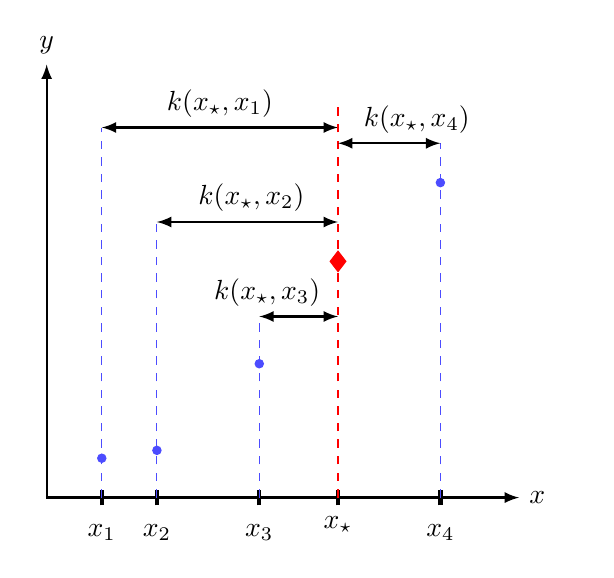
\begin{tikzpicture}[>=latex]
            % This fake axis is added in so that it aligns with the next 
            % two images.
            \begin{axis}[
                    xmin=-0.0,xmax=6.5,
                    ymin=-0.5,ymax=6.5,
                    axis line style={draw=none},
                    tick style={draw=none},
                    yticklabels=\empty,
                    xticklabels=\empty,
                ]
            \end{axis}
            \draw[->,thick] (-0.01,0)--(6,0) node[right]{$x$};
            \draw[->,thick] (0,-0.01)--(0,5.5) node[above]{$y$};

            \draw[-,ultra thick] (0.7,-0.1)--(0.7,0.1) node[below,yshift=-0.3cm]{$x_1$};
            \draw[fill,draw,blue!70] (0.7,0.5) circle[radius=1.5pt];
            \draw[dashed,blue!70] (0.7,0)--(0.7,4.7);
            \draw[<->,thick] (0.7,4.7)--(3.7,4.7) node[above,xshift=-1.5cm]{$k(x_{\star},x_1)$};

            \draw[-,ultra thick] (1.4,-0.1)--(1.4,0.1) node[below,yshift=-0.3cm]{$x_2$};
            \draw[fill,draw,blue!70] (1.4,0.6) circle[radius=1.5pt];
            \draw[dashed,blue!70] (1.4,0)--(1.4,3.5);
            \draw[<->,thick] (1.4,3.5)--(3.7,3.5) node[above,xshift=-1.1cm]{$k(x_{\star},x_2)$};

            \draw[-,ultra thick] (2.7,-0.1)--(2.7,0.1) node[below,yshift=-0.3cm]{$x_3$};
            \draw[fill,draw,blue!70] (2.7,1.7) circle[radius=1.5pt];
            \draw[dashed,blue!70] (2.7,0)--(2.7,2.3);
            \draw[<->,thick] (2.7,2.3)--(3.7,2.3) node[above,xshift=-0.9cm]{$k(x_{\star},x_3)$};

            \draw[-,ultra thick] (3.7,-0.1)--(3.7,0.1) node[below,yshift=-0.2cm]{$x_{\star}$};
            \node[diamond,draw,fill,draw,red,minimum width = 1cm,minimum height = 1.3cm,scale=0.2] (d) at (3.7,3) {};
            \draw[dashed,thick,red] (3.7,0)--(3.7,5);

            \draw[-,ultra thick] (5,-0.1 )--(5,0.1) node[below,yshift=-0.3cm]{$x_4$};
            \draw[fill,draw,blue!70] (5,4) circle[radius=1.5pt];
            \draw[dashed,blue!70] (5,0)--(5,4.5);
            \draw[<->,thick] (3.7,4.5)--(5,4.5) node[above,xshift=-0.3cm]{$k(x_{\star},x_4)$};
        \end{tikzpicture}
    \end{figure}
\end{frame}

\section{The Kernel Trick}

\begin{frame}
    \frametitle{The Kernel Trick}
    \begin{itemize}
        \item Q: How do we get a suitable function $k$ for computing similarity? A: Use the kernel trick!
        \item Suppose we have some inputs $\left[ \text{\PaperPortrait}_1 , \ldots , \text{\PaperPortrait}_n \right]$ (with their corressponding experimental observations $\left[ y_1 , \ldots , y_n \right]$), where $\text{\PaperPortrait}_i$ can take a number of different of form (perhaps a tree data structure or vectors of values).
    \end{itemize}
    \begin{figure}[h]
        \centering
        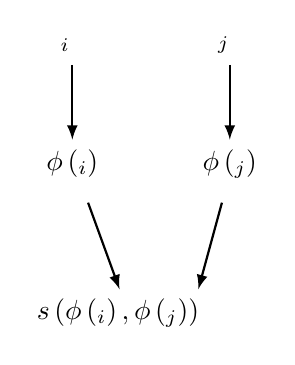
\begin{tikzpicture}[>=latex]
            \node[text width=0.5cm] at (2.1,5) {$\text{\PaperPortrait}_i$};
            \node[text width=0.5cm] at (4.1,5) {$\text{\PaperPortrait}_j$};

            \draw[->,thick] (2,4.75)--(2,3.8) node[below]{$\phi \left( \text{\PaperPortrait}_i \right)$};
            \draw[->,thick] (4,4.75)--(4,3.8) node[below]{$\phi \left( \text{\PaperPortrait}_j \right)$};

            \draw[->,thick] (2.2,3.0)--(2.6,1.9);
            \draw[->,thick] (3.9,3.0)--(3.6,1.9);

            \node[text width=0.5cm] at (1.8,1.6) {$s \left( \phi \left( \text{\PaperPortrait}_i \right), \phi \left( \text{\PaperPortrait}_j \right) \right)$};
        \end{tikzpicture}
        \begin{itemize}
            \item The function $s$ provides us with some notion of similarity between inputs after they've been "transformed" into a nicer form using a {\it feature map} $\phi$.
        \end{itemize}
    \end{figure}
\end{frame}

\begin{frame}
    \frametitle{The Kernel Trick}
    \begin{itemize}
        \item The kernel function $k$ does all this computation is one step so that $k \left( \text{\PaperPortrait}_i , \text{\PaperPortrait}_j \right) = s \left( \phi \left( \text{\PaperPortrait}_i \right), \phi \left( \text{\PaperPortrait}_j \right) \right)$.
        \item Usually we have access to $k$, meaning we can avoid having to construct a feature map $\phi$ and similarity function $s$.
        \item A very common kernel function used is the RBF or Gaussian kernel.
    \end{itemize}
    \vspace*{-\baselineskip}
    \vspace*{-\baselineskip}
    \begin{figure}[h]
        \centering
        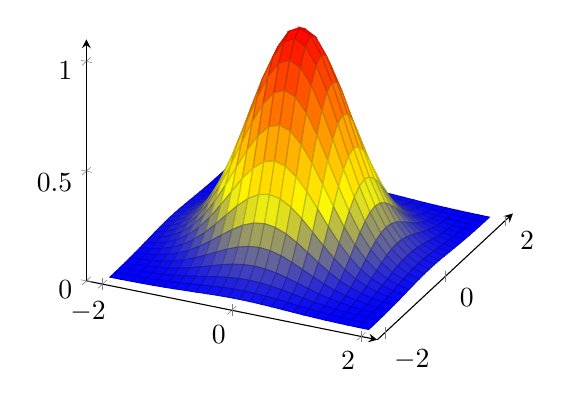
\begin{tikzpicture}

            \begin{axis}[
                    width=7cm,height=7cm,
                    domain=-2:2,
                    xmax=2.25,
                    ymax=2.25,
                    xmin=-2.25,
                    ymin=-2.25,
                    zmax=1.1,
                    axis lines = left,
                    colormap/hot,
                ]

                \addplot3[samples = 25, surf] {exp(-(x^2 + y^2)/1)};

            \end{axis}

        \end{tikzpicture}
    \end{figure}
\end{frame}

\section{Gaussian Processes}

\begin{frame}
    \frametitle{Multi-Variate Gaussian}
    \[
        \mathcal{N} \left(
        \begin{bmatrix}
                \mu_1  \\
                \mu_2  \\
                \mu_3  \\
                \vdots \\
                \mu_n  \\
            \end{bmatrix} ,
        \begin{bmatrix}
                \sigma_{1}^2  & \sigma_{12}^2 & \sigma_{13}^2 & \cdots & \sigma_{1n}^2 \\
                \sigma_{21}^2 & \sigma_{2}^2  & \sigma_{23}^2 & \cdots & \sigma_{2n}^2 \\
                \sigma_{31}^2 & \sigma_{32}^2 & \sigma_{3}^2  & \cdots & \sigma_{3n}^2 \\
                \vdots        &               &               & \ddots & \vdots        \\
                \sigma_{n1}^2 & \sigma_{n2}^2 & \sigma_{n3}^2 & \cdots & \sigma_{nn}^2
            \end{bmatrix}
        \right)
    \]
\end{frame}

\begin{frame}
    \frametitle{Predictions}
    \begin{itemize}
        \item How do we use our data to make predictions with our kernel function?
        \item Within the Gaussian Process paradigm we assume that our data along with the novel point at which we would like to predict form a joint Gaussian distribution.
    \end{itemize}
    \begin{figure}
        \centering
        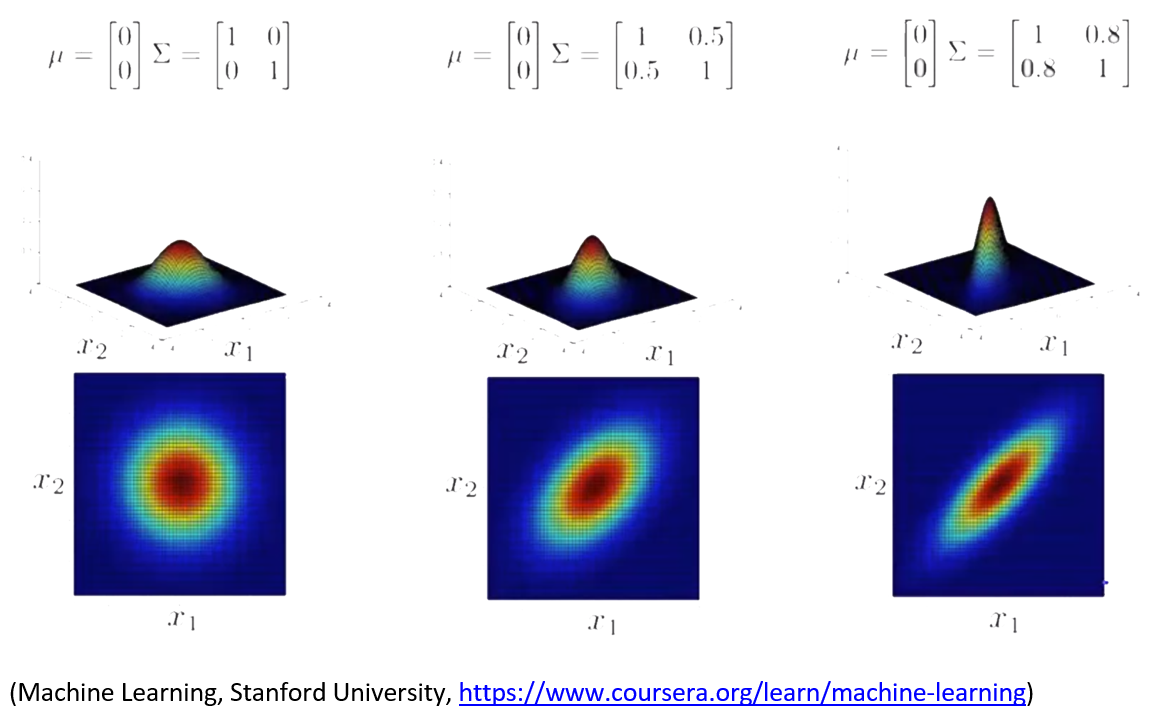
\includegraphics[scale=0.35]{img/multi-var-gaus.png}
    \end{figure}
\end{frame}

\begin{frame}
    \[
        \mathcal{N} \left(
        \begin{bmatrix}
                \mu_1  \\
                \mu_2  \\
                \mu_3  \\
                \vdots \\
                \mu_n  \\
            \end{bmatrix} ,
        \begin{bmatrix}
                \sigma_{11}^2 & \sigma_{12}^2 & \sigma_{13}^2 & \cdots & \sigma_{1n}^2 \\
                \sigma_{21}^2 & \sigma_{22}^2 & \sigma_{23}^2 & \cdots & \sigma_{2n}^2 \\
                \sigma_{31}^2 & \sigma_{32}^2 & \sigma_{33}^2 & \cdots & \sigma_{3n}^2 \\
                \vdots        &               &               & \ddots & \vdots        \\
                \sigma_{n1}^2 & \sigma_{n2}^2 & \sigma_{n3}^2 & \cdots & \sigma_{nn}^2
            \end{bmatrix}
        \right)
    \]
    \vspace{1cm}
    \pause
    \[
        \mathcal{N} \left(
        \begin{bmatrix}
                y_1    \\
                y_2    \\
                \vdots \\
                y_n    \\
                ?      \\
            \end{bmatrix} ,
        \begin{bmatrix}
                k (\bm{x}_1,\bm{x}_1)      & k (\bm{x}_1,\bm{x}_2)      & \cdots & k (\bm{x}_1,\bm{x}_n)      & k (\bm{x}_{1},\bm{x}_{\ast})    \\
                k (\bm{x}_2,\bm{x}_1)      & k (\bm{x}_2,\bm{x}_2)      & \cdots & k (\bm{x}_2,\bm{x}_n)      & k (\bm{x}_{2},\bm{x}_{\ast})    \\
                \vdots                     &                            & \ddots &                            & \vdots                          \\
                k (\bm{x}_n,\bm{x}_1)      & k (\bm{x}_n,\bm{x}_2)      & \cdots & k (\bm{x}_n,\bm{x}_n)      & k (\bm{x}_n,\bm{x}_{\ast})      \\
                k (\bm{x}_{\ast},\bm{x}_1) & k (\bm{x}_{\ast},\bm{x}_2) & \cdots & k (\bm{x}_{\ast},\bm{x}_n) & k (\bm{x}_{\ast},\bm{x}_{\ast})
            \end{bmatrix}
        \right)
    \]
\end{frame}

\begin{frame}
    \begin{itemize}
        \item How do we compute that missing mean within our MVN from the previous slide?
              \pause
        \item We can use the following theorem: (Marginals and conditionals of an MVN), suppose $\bm{x} = [ \bm{x}_1, \bm{x}_2 ]$ is jointly Gaussian with parameters
              \[
                  \bm{\mu} =
                  \begin{bmatrix}
                      \bm{\mu}_1 \\
                      \bm{\mu}_2
                  \end{bmatrix}, \quad
                  \bm{\Sigma} =
                  \begin{bmatrix}
                      \bm{\Sigma}_{11} & \bm{\Sigma}_{12} \\
                      \bm{\Sigma}_{21} & \bm{\Sigma}_{22}
                  \end{bmatrix}
              \]
              then the posterior conditional is given by
              \begin{align*}
                  \bm{x}_2 \mid \bm{x}_1 & \sim \mathcal{N} \left( \bm{x}_2 \mid \bm{\mu}_{2 \mid 1}, \bm{\Sigma}_{2 \mid 1} \right)  \\
                  \bm{\mu}_{2 \mid 1}    & = \bm{\mu}_2 + \bm{\Sigma}_{21} \bm{\Sigma}_{11}^{-1} \left( \bm{x}_1 - \bm{\mu}_1 \right) \\
                  \bm{\Sigma}_{2 \mid 1} & = \bm{\Sigma}_{22} - \bm{\Sigma}_{21} \bm{\Sigma}_{11}^{-1} \bm{\Sigma}_{12}.
              \end{align*}
    \end{itemize}
\end{frame}

\begin{frame}
    \[
        \mathcal{N} \left(
        \begin{bmatrix}
                y_1      \\
                y_2      \\
                \vdots   \\
                y_n      \\
                y_{\ast} \\
            \end{bmatrix} ,
        \begin{bmatrix}
                k (\bm{x}_1,\bm{x}_1)      & k (\bm{x}_1,\bm{x}_2)      & \cdots & k (\bm{x}_1,\bm{x}_n)      & k (\bm{x}_{1},\bm{x}_{\ast})    \\
                k (\bm{x}_2,\bm{x}_1)      & k (\bm{x}_2,\bm{x}_2)      & \cdots & k (\bm{x}_2,\bm{x}_n)      & k (\bm{x}_{2},\bm{x}_{\ast})    \\
                \vdots                     &                            & \ddots &                            & \vdots                          \\
                k (\bm{x}_n,\bm{x}_1)      & k (\bm{x}_n,\bm{x}_2)      & \cdots & k (\bm{x}_n,\bm{x}_n)      & k (\bm{x}_n,\bm{x}_{\ast})      \\
                k (\bm{x}_{\ast},\bm{x}_1) & k (\bm{x}_{\ast},\bm{x}_2) & \cdots & k (\bm{x}_{\ast},\bm{x}_n) & k (\bm{x}_{\ast},\bm{x}_{\ast})
            \end{bmatrix}
        \right)
    \]
    \pause
    \[
        \mathcal{N}
        \begin{pmatrix}
            {
                \begin{bmatrix}
                    \bm{y} \\
                    y_{\star}
                \end{bmatrix}
            }
            , &
            {
                    \begin{bmatrix}
                        \bm{K_{XX}}         & \bm{K_{X_{\star}X}^{\intercal}} \\
                        \bm{K_{X_{\star}X}} & k (\bm{x}_{\ast},\bm{x}_{\ast})
                    \end{bmatrix}
                }
        \end{pmatrix}
    \]
    \pause
    \begin{itemize}
        \item The mean and covariance can then be computed using the theorem from before as
              \begin{align*}
                  y_{\star}                           & = \bm{K_{X_{\star}X}} \bm{K_{XX}}^{-1} \bm{y}                                                             \\
                  \mathbb{V} \left[ y_{\star} \right] & = k (\bm{x}_{\ast},\bm{x}_{\ast}) - \bm{K_{X_{\star}X}} \bm{K_{XX}}^{-1} \bm{K_{X_{\star}X}}^{\intercal}.
              \end{align*}
              \pause
        \item Another way of looking at the prediction is seeing it as a linear combination of $n$ kernel evaluations centered at the input $\bm{x}_{\star}$
              \[
                  y_{\star} = \sum_{i=1}^{n} \alpha_i k \left( \bm{x}_i , \bm{x}_{\star} \right)
              \]

    \end{itemize}
\end{frame}

\begin{frame}
    \frametitle{Unoptimized GPR}
    {\centering
        \begin{minipage}{.9\linewidth}
            \begin{algorithm}[H]
                \caption{Unoptimized GPR}
                \SetAlgoLined
                \DontPrintSemicolon
                \SetKwInOut{Input}{input}\SetKwInOut{Output}{output}

                \Input{Observations $\bm{X}, \bm{y}$ and a test input $\bm{x}_{\star}$.}
                \Output{A prediction $y_{\star}$ with its corresponding variance $\mathbb{V} \left[ y_{\star} \right]$.}
                \BlankLine
                $\bm{L} = \operatorname{cholesky} \left( \bm{K_{XX}} \right)$\;
                $\bm{\alpha} = \operatorname{lin-solve} \left( \bm{L}^{\intercal} , \operatorname{lin-solve} \left( \bm{L}, \bm{y} \right) \right)$\;
                $y_{\star} = \bm{K_{x_{\star} X}} \bm{\alpha}$\;
                $\bm{v} = \operatorname{lin-solve} \left( \bm{L}, \bm{K_{x_{\star} X}} \right)$\;
                $\mathbb{V} \left[ y_{\star} \right] = k (\bm{x}_{\ast},\bm{x}_{\ast}) - \bm{v}^{\intercal} \bm{v}$\;
                \Return{$y_{\star} , \mathbb{V} \left[ y_{\star} \right]$}
                \BlankLine
            \end{algorithm}
        \end{minipage}
        \par
    }
\end{frame}

\section{Applications}

\begin{frame}[fragile]
    \frametitle{Implementation}

    \begin{minted}{python}
    def gp_reg_pred(X_train, Y_train, x_pred, sigma):
        n, d = X_train.shape
        # Create the Gram matrix corresponding to the training data set.
        K = exact_kernel(X_train, sigma=sigma)
        # Noise variance of labels.
        s = np.var(Y_train.squeeze())
        L = np.linalg.cholesky(K + s*np.eye(n))
        # Compute the mean at our test points.
        Lk = np.linalg.solve(L, exact_kernel(X_train, x_pred, sigma=sigma))
        Ef = np.dot(Lk.T, np.linalg.solve(L, Y_train))
        # Compute the variance at our test points.
        K_ = exact_kernel(x_pred, sigma=sigma)
        Vf = np.diag(K_) - np.sum(Lk**2, axis=0)
        return Ef, Vf
    \end{minted}

\end{frame}

\begin{frame}
    \frametitle{$\sin$ Function Prediction with Added Noise}

    \begin{figure}
        \centering
        \begin{adjustbox}{width=0.9\textwidth}
            \includegraphics[scale=1]{img/sin_eg.png}
        \end{adjustbox}
    \end{figure}
\end{frame}

\begin{frame}
    \frametitle{Stock Market Prediction}

    \begin{figure}
        \centering
        \begin{adjustbox}{width=0.9\textwidth}
            \includegraphics[scale=1]{img/stock_eg.png}
        \end{adjustbox}
    \end{figure}
\end{frame}

\end{document}